In this section, we examine our experimental results to address the above research questions over the performance of our algorithm.

\begin{figure}[t]
 \centering
  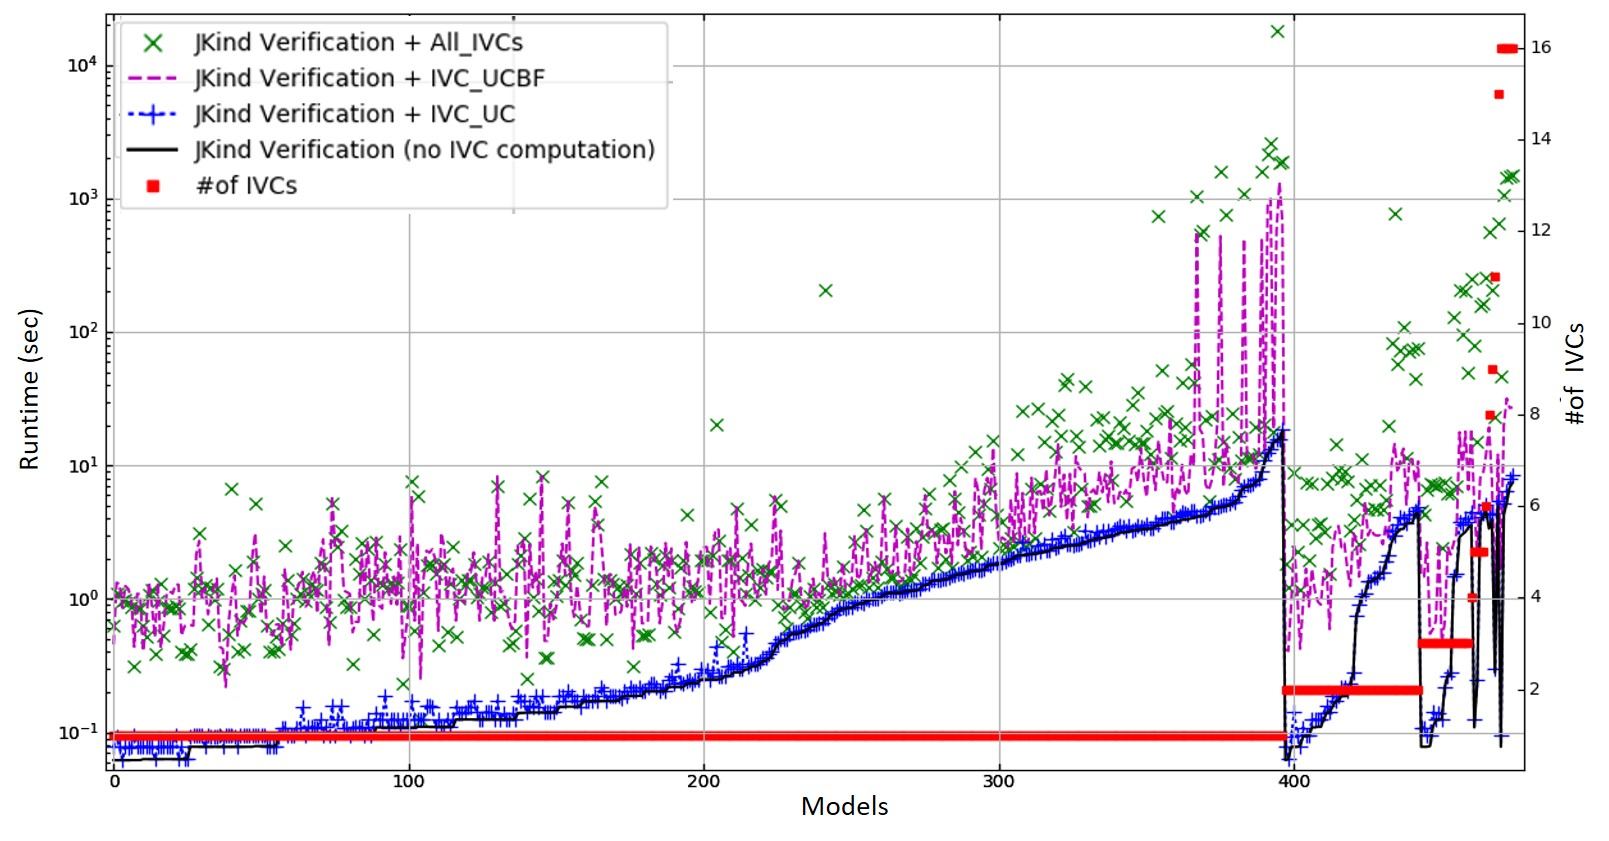
\includegraphics[width=\textwidth]{figs/performance.jpg}
  \label{fig:performance}
  \vspace{-0.2in}
  \caption{Runtime of \aivcalg, \ucbfalg, and \ucalg ~algorithms}
\end{figure}
\vspace{0.1in}
\textbf{RQ1)} We measured the performance overhead of the algorithms over the time
necessary to find a proof using inductive model checking. Fig. \ref{fig:performance}
 allows a visualization of the  overhead  of the \aivcalg ~algorithm  in  comparison  with \ucalg ~and \ucbfalg.
 In the figure, the models are ranked along the x-axis by the number of IVCs found by \ucalg ~per model.
 Table \ref{tab:runtime} and Table \ref{tab:overhead} also provide a summary of the computation time and the overhead of different algorithms.
 As it can be seen, the \ucalg ~algorithm imposes a negligible overhead to the proof time and is quite fast, whereas \ucbfalg ~algorithm adds a substantial penalty in order to find a single IVC.
 The \aivcalg ~algorithm is able to outperform the \ucbfalg ~in a lot of cases,
 or perform approximately the same.
 Note that the \aivcalg ~algorithm could have had better (worse) performance
 if timeout had been set lower (higher), which caused the average runtime (overhead) of the \aivcalg ~shown in Table \ref{tab:runtime} (Table \ref{tab:overhead}) to be $\thicksim 3$ times more than \ucbfalg .


\begin{table}
  \caption{Runtime of different computations}
   \vspace{-0.1in}
  \centering
  \begin{tabular}{ |c||c|c|c|c| }
    \hline
      runtime (sec)& min & max & mean & stdev \\[0.5ex]
    \hline\hline
    \emph{\small{proof-time}}    & 0.047 & 14.617 & 1.299 & 1.940 \\[0.5ex]
    \aivcalg    & 10.125 & 2375.058& 58.884 & 256.529 \\[0.5ex]
    \ucbfalg &   0.248 & 1323.515 &  17.247& 104.838\\[0.5ex]
    \ucalg&  0.0  & 1.422  & 0.084 & 0.184 \\[0.5ex]
    \hline
  \end{tabular}
  \label{tab:runtime}
\end{table}

\begin{table}
  \caption{Overhead of different algorithms}
   \vspace{-0.1in}
  \centering
  \begin{tabular}{ |c||c|c|c|c| }
    \hline
     algorithm & min & max & mean & stdev \\[0.5ex]

    \hline
    \aivcalg   & 13.642\% & 101034.615\% & 2544.399\% & 7764.159\% \\[0.5ex]
    \ucbfalg &   14.092\% & 111124.432\% &  882.018\% & 1512.071\%\\[0.5ex]
    \ucalg&  0.00\%  & 100.00\%   & 10.226\% & 11.718\% \\[0.5ex]
    \hline
  \end{tabular}
  \label{tab:overhead}
\end{table}

%\takeaway{Computing all minimal Inductive Validity Cores with the \aivcalg ~algorithm is as nearly expensive as computing one single minimal Inductive Validity Core with the \ucbfalg  ~algorithm.
%\ela{Ela: is that fair to say??}}
\vspace{0.1in}
\textbf{RQ2)} The structure of the model and specification can play a part in how well \aivcalg ~performs.
Therefore, we would like to examine whether or not there is a relationship between the performance and the size of the model, proof-time, and the diversity of IVCs. A graph showing the size of each model (determined by the number of equations in the model) and the number of IVCs
 along with the running time of \aivcalg ~and normal verification time is shown in Fig \ref{fig:modelsize}. In the figure, the models are ranked along the x-axis by their size. The picture shows that as models get larger, it is more likely for the \aivcalg ~algorithm to take more time to complete. However, there is no straightforward relationship between the performance and the number of IVCs. It can be expected that the running time of the \aivcalg ~algorithm goes higher when verification takes more time.

 \begin{figure}[t]
 \centering
  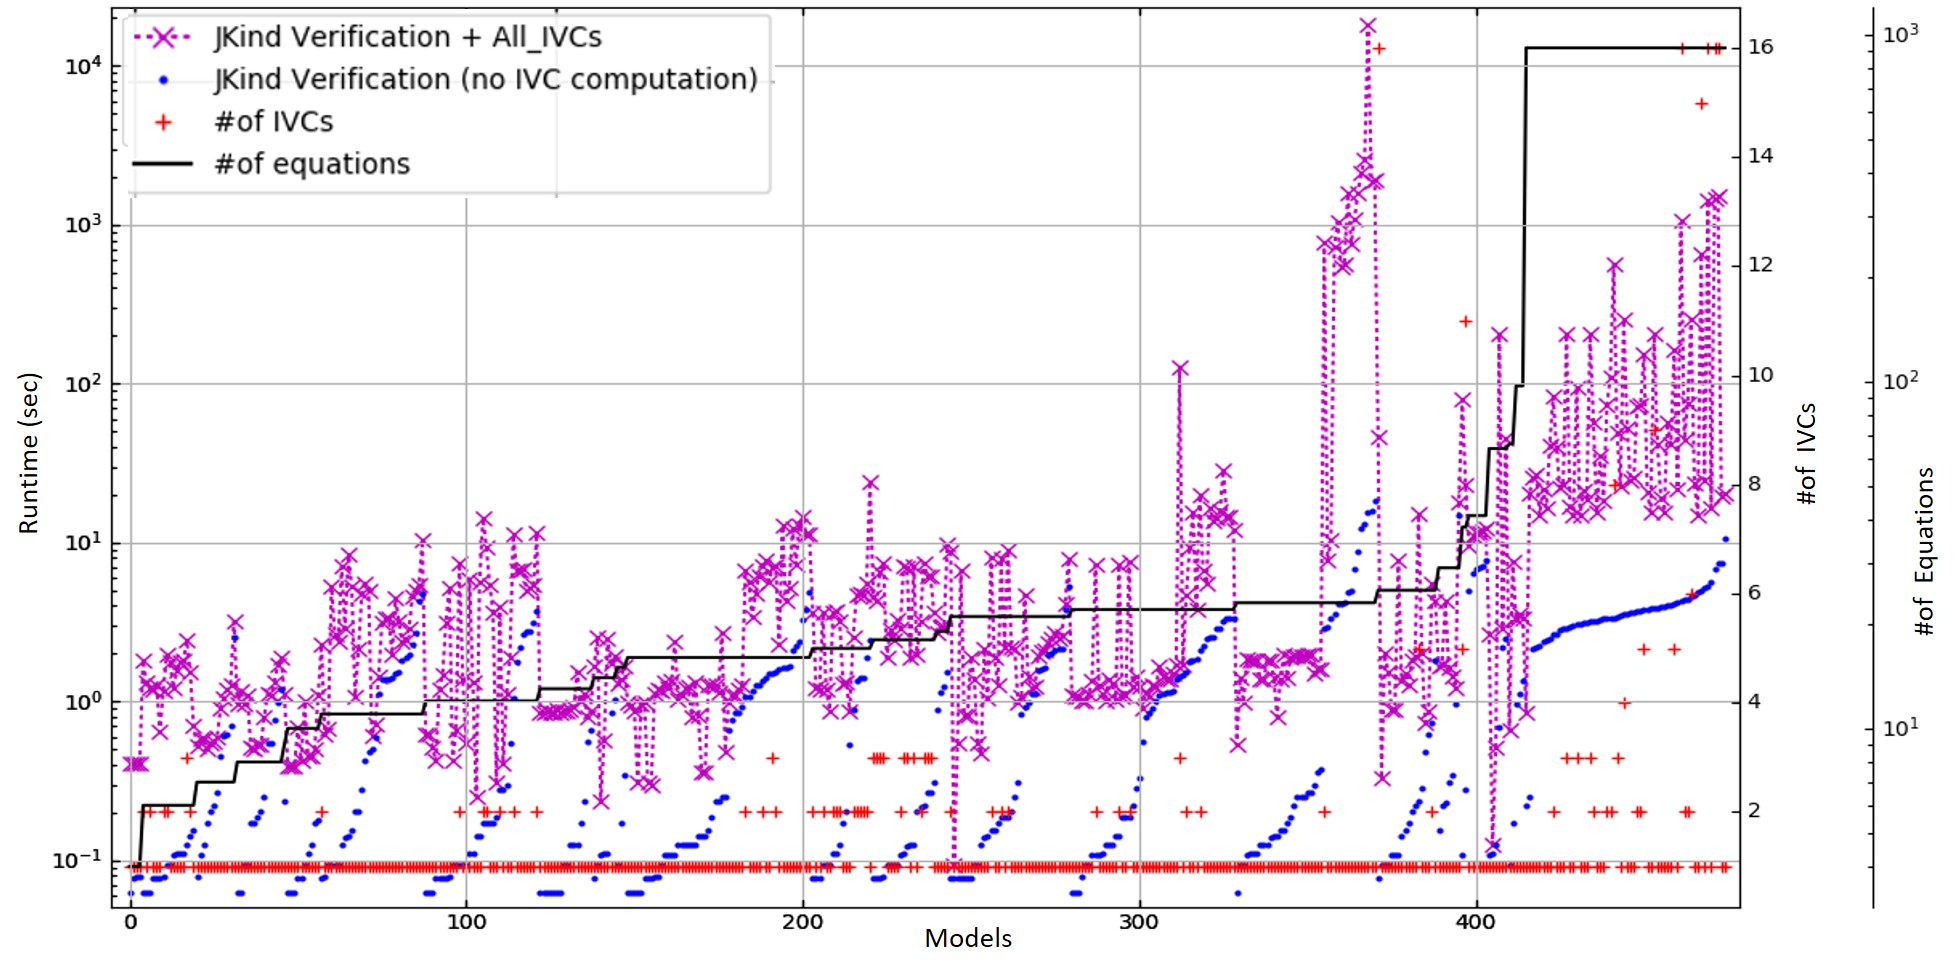
\includegraphics[width=\textwidth]{figs/numofeq.jpg}
  \label{fig:modelsize}
  \vspace{-0.2in}
  \caption{Runtime of \aivcalg ~along with the model size and number of IVCs}
\end{figure}
\vspace{0.1in}
\textbf{RQ3)} Table \ref{tab:ivcsize} compares
the  minimum,  maximum,  average,
and standard deviation of the size of the IVCs computed by the different algorithms.
For the \aivcalg ~algorithm, the  minimum,  maximum,  average,
and standard deviation of the size of the IVCs per model is calculated, and then again, these four measures are calculated among all models.
As for the \texttt{minimum IVC} row, the four measures are calculated among the size of the minimum IVC generated by \aivcalg ~for each model. 
The size of IVCs computed by \ucalg ~and \ucbfalg ~are quite close to each other. It means the \ucalg ~algorithm computes IVCs that are very close to the minimal ones obtained from the \ucbfalg , which makes the \ucalg ~algorithm a reasonable choice for the \getivc ~procedure in Algorithm \ref{alg:aivc}
although it does not guarantee minimality.
Fig. \ref{fig:ratio} also demonstrates that average cost of \aivcalg ~per IVC is very close to average cost of finding one IVC by \ucbfalg. Given the fact that the size of IVCs generated by \ucalg ~is very close to the ones generated by \ucbfalg, makes the \ucalg ~algorithm
more efficient for the \getivc ~procedure.

\begin{table}
  \caption{Size of IVCs from different computations}
   \vspace{-0.1in}
  \centering
  \begin{tabular}{ |c||c|c|c|c| }
    \hline
     algorithm & min & max & mean & stdev \\[0.5ex]

    \hline
    \aivcalg   & 1 & 159 & 12.462 & 1.1684 \\[0.5ex]
    \ucalg   & 1 & 141 & 12.754 & 16.000 \\[0.5ex]
    \ucbfalg &   1 & 141 &  12.185 & 16.107\\[0.5ex]
    \texttt{minimum IVC} & 1  & 134  & 12.078 & 15.550 \\[0.5ex]
    \hline
    \end{tabular}
  \label{tab:ivcsize}
\end{table}

 \begin{figure}
 \centering
  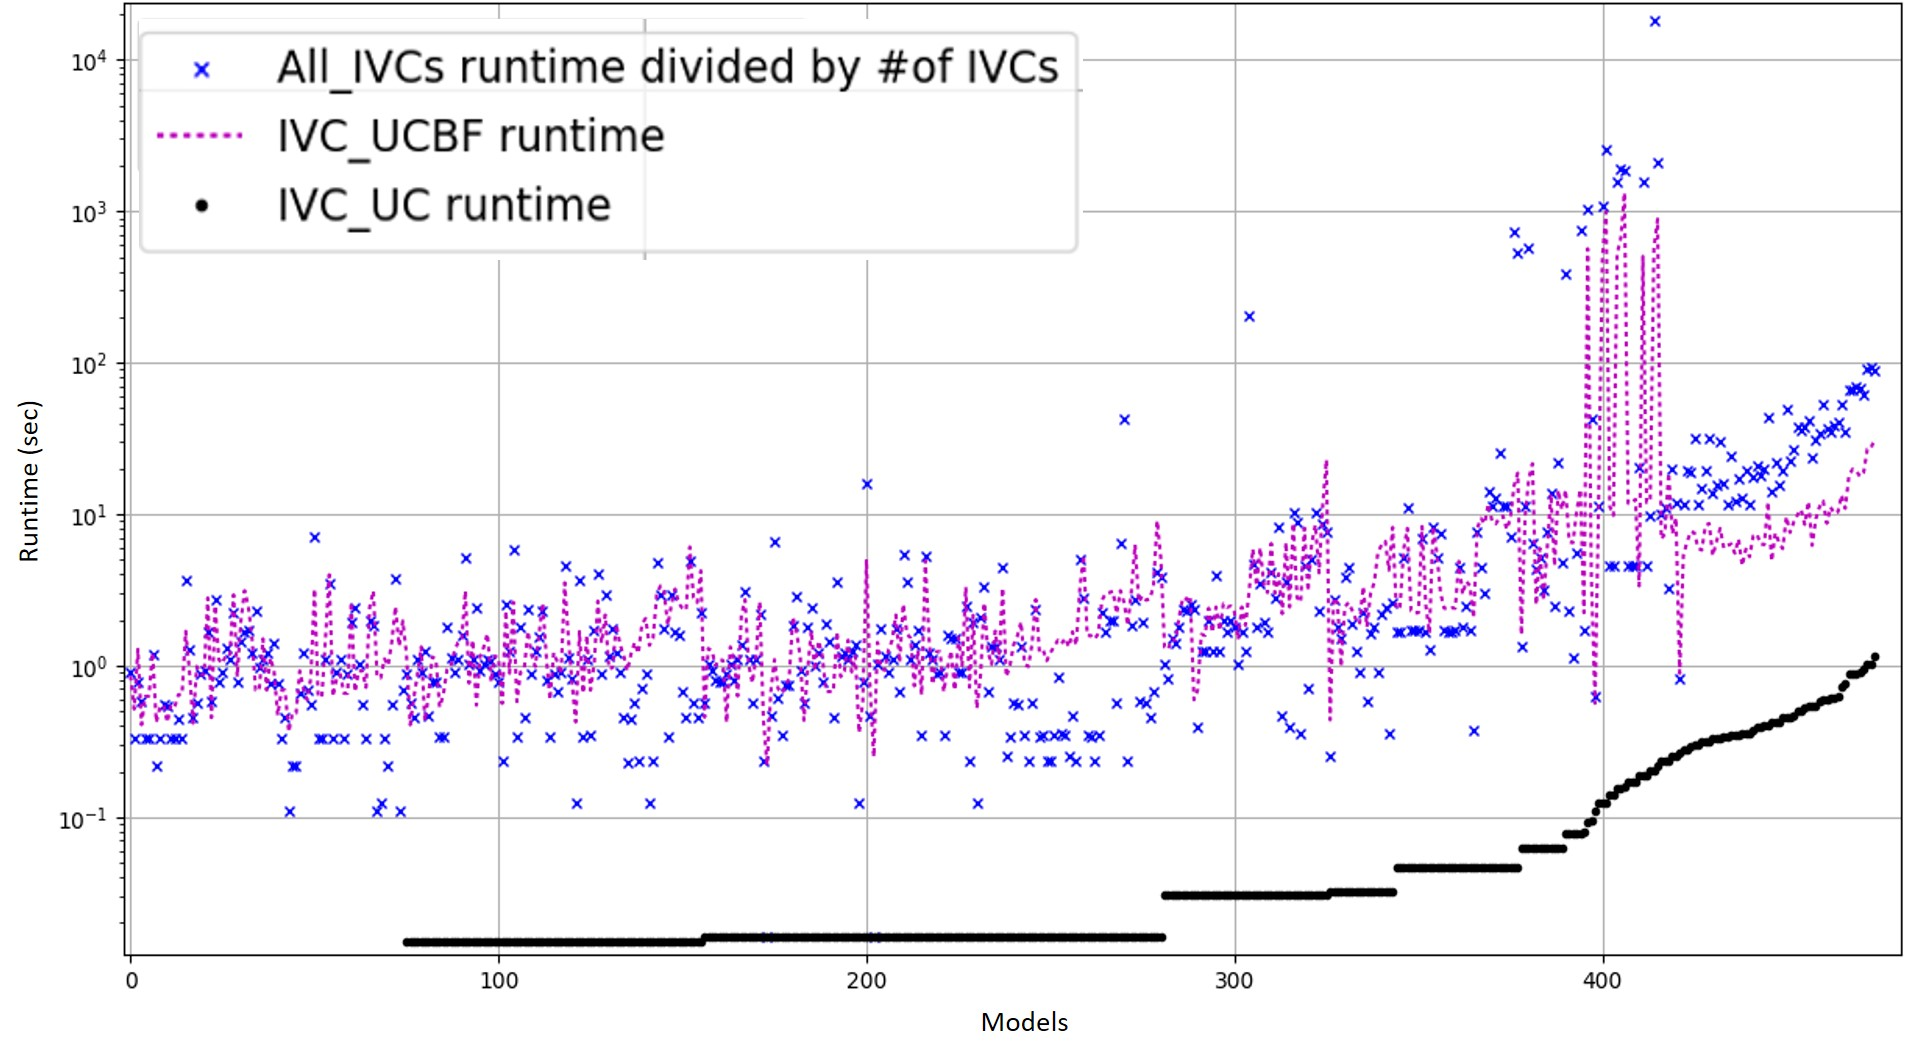
\includegraphics[width=\textwidth]{figs/ratio.jpg}
  \label{fig:ratio}
  \vspace{-0.2in}
  \caption{Runtime of \aivcalg ~along divided by the number of IVCs vs the runtime of other computations}
\end{figure}

\vspace{0.1in}
\textbf{RQ4)} In the benchmarks, there have been
several models containing undecidable cases which affected the average
performance of \aivcalg ~reported in Table \ref{tab:runtime}. Moreover, such cases also influence the minimality of the IVCs computed by \aivcalg. It is also possible that an iteration of
the \texttt{while} loop in Algorithm \ref{alg:aivc} times out while
the adequacy of the subset under examination is decidable in general.
We were interested in determining how often it is possible to come across such cases in our benchmarks. Size of IVCs obtained from different algorithms is shown in Fig. \ref{fig:min}.
As you can see, there are 14 cases among 476 models for which the size of
 minimum IVC computed by the \aivcalg ~is bigger than the size of the minimal IVC
 generated by the \ucbfalg ~algorithm.
 \begin{figure}
 \centering
  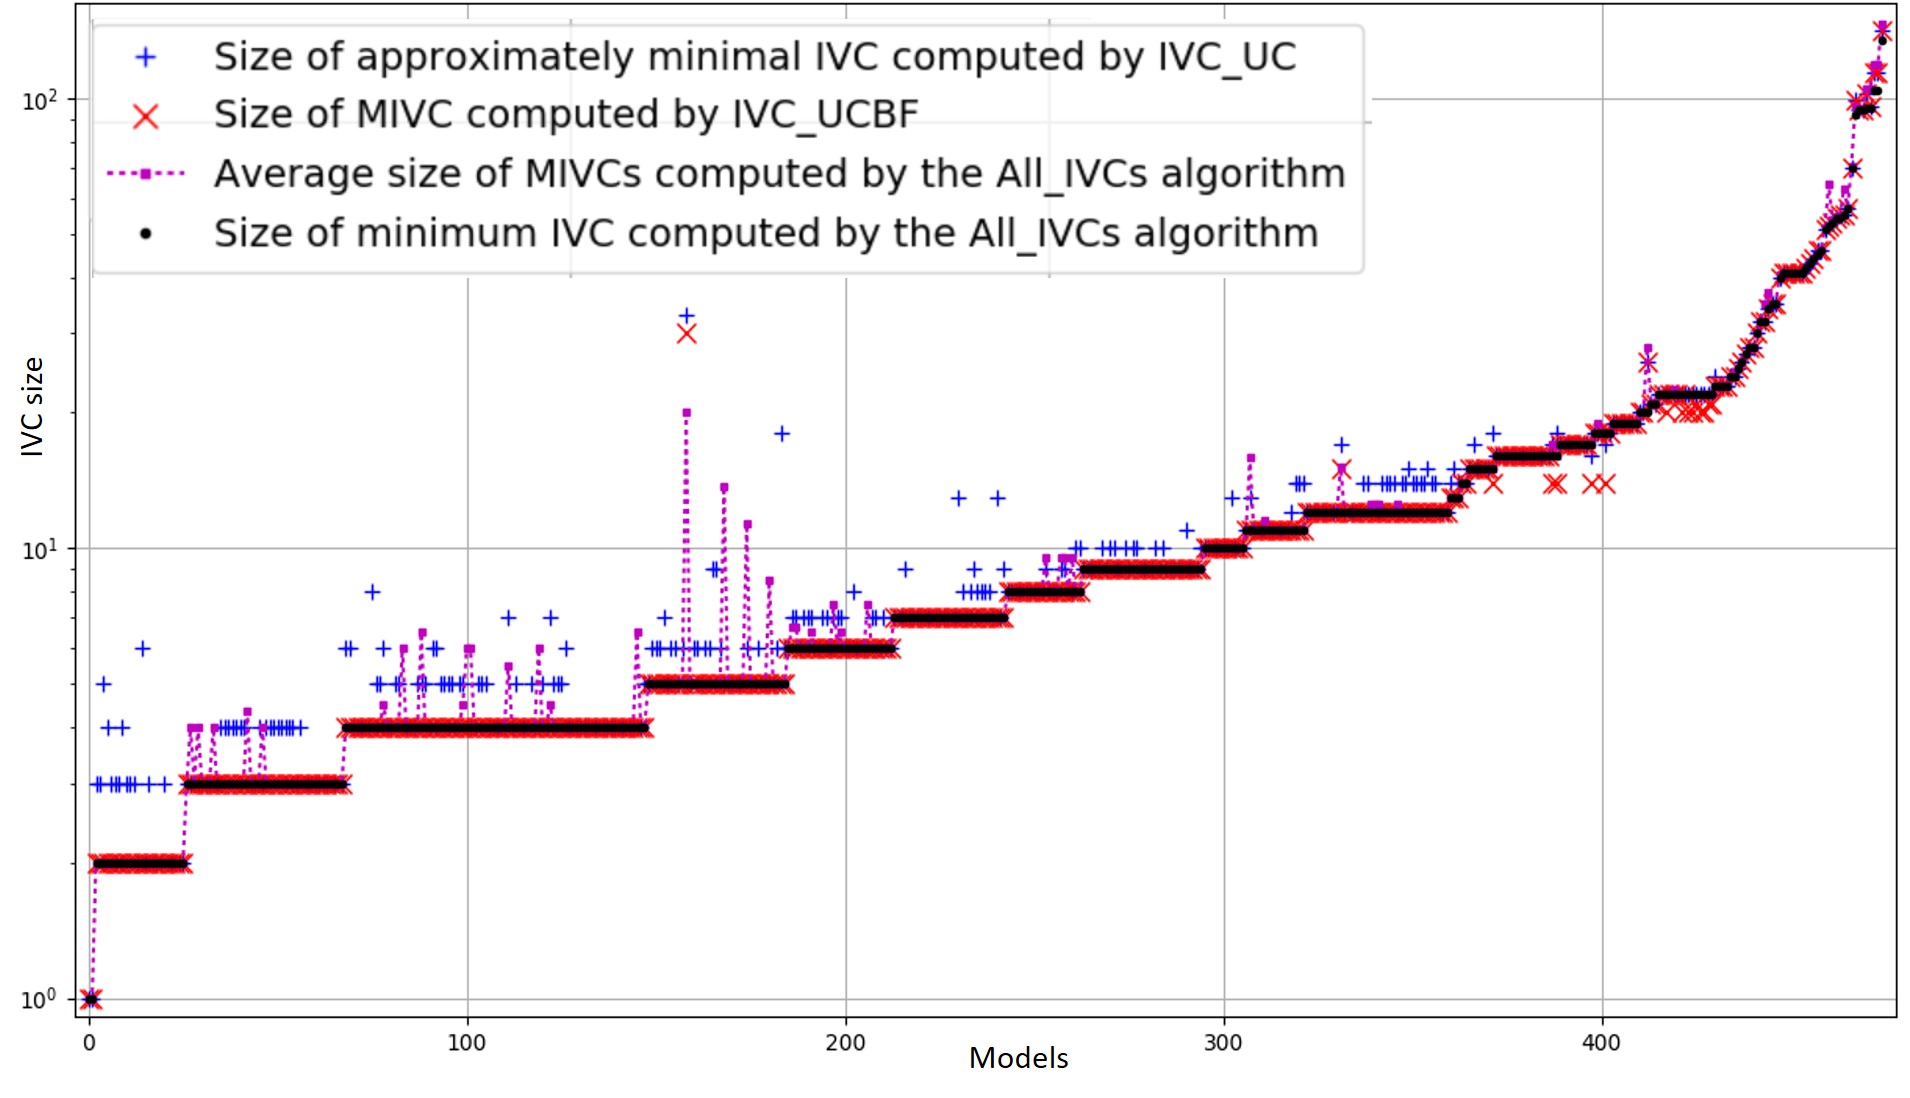
\includegraphics[width=\textwidth]{figs/min.jpg}
  \label{fig:min}
  \vspace{-0.2in}
  \caption{Size of IVCs obtained from different computations}
\end{figure}
